\graphicspath{{./assets/}}
\setcounter{mtc}{1}
\chapter{Generalized context of the project }
\fancyhead[R]{\ungaramond\small\textbf{Chapter I. Generalized context of the project}}
\minitoc
\newpage
\section*{Introduction}
The Generalized context of a project is a crucial aspect that outlines the scope, purpose, and objectives of the project. For an end of study project in the fields of cloud computing and DevSecOps, the Generalized context of the project is critical in providing a comprehensive understanding of the project's goals and expected outcomes. 

Cloud computing is a technology that enables users to access computing resources, such as servers, storage, applications, and services, over the internet on a pay-per-use basis. DevSecOps, on the other hand, is an approach that integrates security into the software development and operations process. 

This chapter provides a comprehensive overview of the project's context, including the problem statement, objectives, and scope. It aims to provide a clear understanding of the project's purpose and the expected outcomes

\section{Overview on the host organization  }

\subsection{Company Background }
Systnaps is a technology company based in Paris, France that specializes in providing innovative software solutions to businesses across various industries. It prides itself with the expertise in areas such as data analytics, artificial intelligence, machine learning, and cloud computing. The following figure illustrates the company logo: 

\begin{figure}[!ht]\centering

\includegraphics[width=0.5\textwidth,angle=00]{assets/fa.png}
\caption{Systnaps Logo}
\end{figure}

Huxium, an affiliate of Systnaps is a technology company that specializes in providing customized software solutions to businesses across various industries. 


\begin{figure}[!ht]\centering

\includegraphics[width=0.5\textwidth,angle=00]{assets/fb.png}
\caption{Huxium Logo}
\end{figure}


 \subsection{Mission and Vision }

Systnaps was founded with the mission of helping businesses harness the power of technology to improve their operations, enhance customer experiences, and drive growth. They offer a range of services to meet the diverse needs of their clients, including custom software development, application maintenance and IT consulting. 

\subsection{Core Services or Products }

The core services of Systnaps in the data management space include: 
\begin{itemize}[label={--}]
    \item Database Management: Systnaps offers services to help businesses manage their databases, ensuring their data is secure and available when needed. This includes tasks such as database administration, performance optimization, and disaster recovery. 

\item Data Integration: Systnaps offers services to help businesses integrate and manage their data across multiple systems and platforms. This includes tasks such as data migration, data warehousing, and data synchronization. 

\item Big Data: Systnaps offers services to help businesses manage and analyze large volumes of data, often referred to as "big data". This includes tasks such as data processing, data visualization, and machine learning. 

\item  Data Governance: Systnaps offers services to help businesses ensure that their data is being managed in compliance with regulatory and legal requirements. This includes tasks such as data privacy and security, data classification, and data retention. 

 \end{itemize}

\subsection{Market Position and notable clients }

While they do not have a significant global presence, they have established themselves as a reputable player in the French IT market. 

Systnaps has worked with clients across a range of industries, including finance, healthcare, and media. The following figure showcases some of the current clients: 


\begin{figure}[!ht]\centering
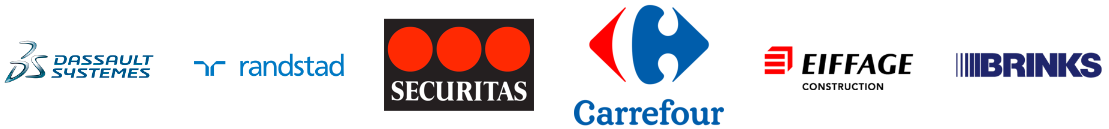
\includegraphics[width=0.8\textwidth,angle=00]{assets/fc.png}
\caption{Company clients}
\end{figure}


\section{Project description }

Our end of studies project involves designing and implementing, on the cloud, a complete platform as a service (PaaS) solution that incorporates a range of services related to networking, storage, and automation. 

Specifically, this project involves designing and implementing a PaaS platform that includes a range of networking services, such as load balancing, ingress, and authentication/authorization, which are essential for managing traffic flow and ensuring secure access to the platform. 

The project also involves implementing a distributed and redundant storage backend that includes both object and block storage to ensure reliable and scalable storage capabilities. 

In addition, the PaaS platform includes highly available and replicated database storage services to provide reliable and consistent data access for users. 

The project also includes implementing utility services that help store artifacts, such as a private registry, and automate CI/CD operations to streamline the deployment process. 


Finally, the PaaS platform includes a resilient and efficient disaster recovery strategy to ensure that the platform can quickly recover from any unplanned downtime or service interruptions. 

Overall, this end of studies project demonstrates a thorough understanding of cloud computing and DevSecOps principles and the ability to design and implement a comprehensive PaaS platform that incorporates a range of essential services to support modern application development and deployment. 

\section{Analysis of existing processes }

The existing infrastructure is built on a few monolithic virtual private servers and are using Docker Compose for container orchestration. The infrastructure contains multiple Docker Compose stacks that are used for different purposes. These stacks include: 
\begin{itemize}[label={--}]
\item Docker Compose stacks of applications in development: These stacks contain the necessary applications for software development, such as code editors, compilers, and development frameworks. 

\item A self-hosted instance of GitLab: This stack contains a self-hosted instance of GitLab, which is used for version control, continuous integration, and continuous deployment (CI/CD) of the applications. 

\item A self-hosted instance of Nextcloud: This stack contains a self-hosted instance of Nextcloud, which is a file hosting and sharing platform. It is used to store and share files related to the application development. 

\item A reverse proxy stack: This stack contains three different Docker images - acme-companion, docker-gen, and nginx - and is used as a reverse proxy for the application. Nginx is a web server that is used to route traffic to the application, while acme-companion and docker-gen are used to generate SSL/TLS certificates and automatically update the Nginx configuration. 
\end{itemize}

The use of Docker Compose to manage containers provides a lightweight and scalable infrastructure for application development. However, using monolithic virtual private servers can lead to a lack of scalability and make it difficult to maintain the infrastructure. Additionally, running all the services on a single server can create a single point of failure and increase the risk of downtime. 

\section{Constructive criticism on existing processes} 

Based on cloud computing and DevOps practices, there are several constructive criticism that can be made regarding this infrastructure with the following components: 

\begin{itemize}[label={--}]

\item The use of Docker Compose for application orchestration is suitable for small-scale projects or individual development environments, but it becomes difficult to manage and maintain as the number of services and containers increases. Kubernetes provides a more scalable and efficient solution for container orchestration and management. 

\item The lack of a distributed storage backend can lead to data loss or inconsistency in case of node failures. Kubernetes provides several built-in options for distributed storage, such as persistent volumes, stateful sets, and storage classes. 

\item The absence of an authorization and authentication backend can result in security vulnerabilities and unauthorized access to sensitive data. Kubernetes provides several options for authentication and authorization, such as role-based access control (RBAC), webhook token authentication, and client certificate authentication. 

\item The lack of a disaster recovery strategy can lead to significant downtime and data loss in case of unforeseen events such as natural disasters or system failures. Kubernetes provides several options for disaster recovery, such as backup and restore mechanisms, failover and recovery strategies, and multi-zone deployments. 

\item The use of large and inefficient container images can result in slower deployment times, increased storage requirements, and decreased performance. DevOPS best practices help a great deal in streamlining application development and delivery, and Kubernetes provides several features such as image caching, rolling updates, and horizontal scaling, which can help optimize container image management and deployment. 

\end{itemize}

In summary, the adoption of Kubernetes and the implementation of cloud computing and DevOps best practices can greatly improve the scalability, reliability, security, and performance of an IT ecosystem. 

\section{Problem statement }

In today's fast-paced business environment, the company is looking to leverage cloud computing and DevSecOps practices to gain a competitive edge.  

However, building and managing a PaaS platform that provides reliable and scalable infrastructure services is a complex and challenging task. The lack of a well-designed and integrated PaaS platform can lead to increased costs, inefficient resource utilization, and security vulnerabilities. 

The objective of this project is to design, build and implement a PaaS platform that provides a complete set of infrastructure services, including networking, storage, database, and utility services, along with a resilient and efficient disaster recovery strategy. The platform will also incorporate DevSecOps practices to ensure security and compliance with industry standards. 

The main challenge of this project is to ensure the scalability, availability, and security of the PaaS platform while providing a simple and intuitive user experience for developers. This requires a deep understanding of cloud computing and DevSecOps practices, along with expertise in networking, storage, database, and utility services. 

The successful implementation of this project will enable the company to accelerate their digital transformation journey, reduce operational costs, and improve their overall business agility. 

 

\section{Ideation and proposed solutions} 

The company has decided to explore the possibility of moving to a cloud-based infrastructure to increase scalability, availability, and security. After analyzing various options, we have decided to propose a self-managed PaaS platform based on Kubernetes that contains the following components: 

\begin{itemize}[label={--}]

\item Networking services: The networking services will be provided by MetalLB for layer 4 load balancing, Traefik as an ingress controller, and Cert-manager for TLS provisioning. The platform will also use Authelia, OpenLDAP, and Redis for authentication/authorization. 

\item A Storage backend: The storage backend will be provided by Ceph, which is a distributed and redundant storage backend for both object and block storage. This will ensure that data is highly available and can be easily scaled. 

\item Highly available and replicated database storage services: The platform will use both MongoDB and PostgreSQL as highly available and replicated database storage services for both the relational and document models. This will provide the necessary data persistence and redundancy required for a PaaS platform. 

\item DevSecOPS utility services: The platform will use several utility services to help store artifacts, automate CI/CD operations, and improve code quality. These services include Jenkins as the CI/CD orchestrator, ArgoCD as the CD controller, SonarQube for code scanning, Harbor as a private registry, and Jenkins pipelines to automate building applications, scanning, and delivery. 

\item Disaster recovery strategy: The platform will have a resilient and efficient disaster recovery strategy that uses Velero to back up Kubernetes related objects and proprietary Python programs to backup database data. This will ensure that the platform is highly available, even in the event of a disaster. 

\end{itemize}

Overall, the proposed solution will provide a highly available, scalable, and secure PaaS platform that can meet the company's needs for application development and deployment. The platform will also have a robust disaster recovery strategy, which will ensure business continuity in the event of an outage.  


\newpage  % if no new page table will not be in the good place
\section{Project management }
\subsection{Comparative research }

\begin{table}[h!]
\center
\begin{tabular}[b]{|m{3cm}|m{4cm}|m{4cm}|m{4cm}|}
\hline
\rowcolor{white}
 & Waterfall (V model) 
 & Agile   & DevOPS  \\
\hline
 Lifecycle  
& Linear software development approach 
& Incremental and iterative sprint cycles. 
& Uses automation techniques to enable continuous deployment of change. \\
\hline
 Automation level  
& Low 
& Varied 
& High 
 \\
\hline
 Delivery of value 
& Slow (Scale : months) 
& Rapid (daily/weekly) 
& Continuous  \\
\hline
 Responsiveness to business needs 
& Extremely limited 
& Responsive 
& Highly responsive   \\
\hline
 Collaboration 
& Low: teams operate in functional silos 
& Improved: short dev cycles 
& High: cross-functional teams are involved from project start. \\
\hline
Quality 
& Low: issues are only identified after tests 
& Improved: issues are identified after every sprint 
& High: Unit testing and code quality checks are performed during development. \\
\hline
 Risk 
& Increases as project development progresses 
& Decreases as project development progresses 
& Decreases as project development progresses \\
\hline
\end{tabular}
\caption{ comparative study}
\textcolor{white}{I} \label{tab:tab-m}
\end{table}

Based on the previous comparative study, it is apparent that the approach most suited to our use case is one that helps improve collaboration, reduce context-switching, introduce automation, and enable observability and monitoring. 

\subsection{Agile devSecOPS }

When evaluating devSecOPS as a practice and Agile as a delivery approach, it is important to note that they are not mutually exclusive. In spite of the evident differences between DevSecOPS and the Agile methodology, their overall goal of increasing speed and delivering quality software is similar in nature and together they produce great products and improve the software development. 

The following figure showcases an overview of the process and the key DevSecOPS roles. 

\begin{figure}[!ht]\centering
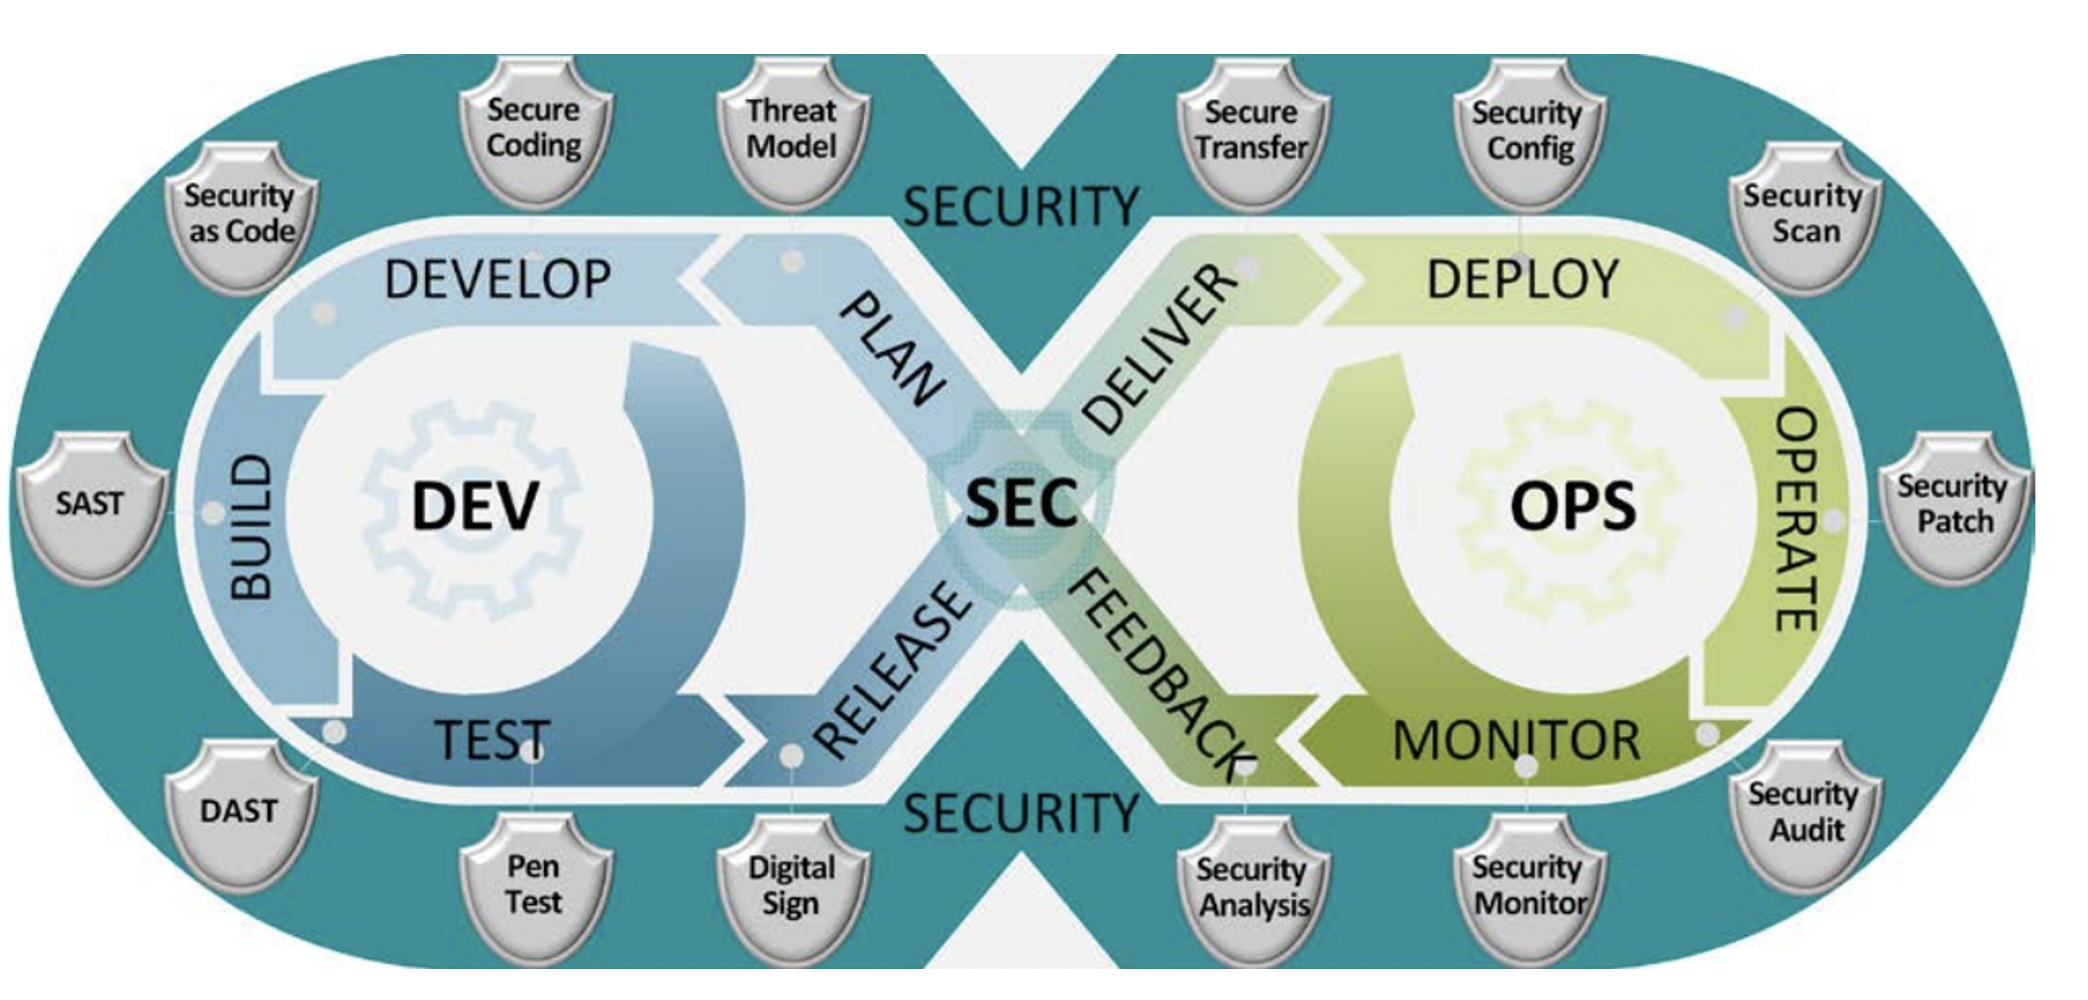
\includegraphics[width=0.8\textwidth,angle=00]{assets/f1.png}
\caption{Process overview}
\label{fig:processOverview}
\end{figure}


\paragraph{DevSecOPS Evangelist:} 
Usually the DevSecOPS team leader, he focuses on promoting the DevSecOPS advantages, identifying and quantifying companies’ benefits deriving from a higher agility. 

\paragraph{Release Manager:} 
The product stability manager which is basically the product owner. He cares about the product’s management and coordination. 

\paragraph{Automation Architect: }
Provides a complete automation role involving the DevSecOPS and Cloud solutions. He is an integration specialist that ensures the high availability of the pre-production and production systems. 

\paragraph{Software Developer/Tester:}
DevSecOPS developers are not responsible only for the transformation of new requirements into code, they also have to deal with testing, distribution and continuous monitoring processes.

\paragraph{Security Engineer: }
The DevSecOPS approach implements security by design.


\section*{Conclusion}

In this chapter, we started by introducing the project's background, highlighting the need for the project, and discussing the current state of the art. This was followed by a detailed description of the problem statement, which identifies the specific issue that the project aims to address. The ideation phase provided us with specific, measurable, achievable, relevant, and time-bound (SMART) objectives to ensure that they are attainable and can be evaluated. 

Overall, we gathered a rough understanding of the project's context, which is essential to understand the project's purpose, scope, and expected outcomes. It sets the foundation for the rest of the project and provides a clear roadmap for achieving the project's objectives.